\documentclass[11pt,addpoints,answers]{exam}
%\documentclass[11pt]{article}
\usepackage[margin=1in]{geometry}
\usepackage{amsmath, amsfonts}
\usepackage{enumerate}
\usepackage{graphicx}
\usepackage{titling}
\usepackage{url}
\usepackage{xfrac}
% \usepackage{fancyhdr} % CONFLICTS with the exam class
\usepackage{geometry}
\usepackage{graphicx}
\usepackage{natbib}
\usepackage{amsmath}
\usepackage{amssymb}
\usepackage{amsthm}
\usepackage{paralist}
\usepackage{epstopdf}
\usepackage{tabularx}
\usepackage{longtable}
\usepackage{multirow}
\usepackage{multicol}
\usepackage[colorlinks=true,urlcolor=blue]{hyperref}
\usepackage{fancyvrb}
\usepackage{algorithm}
\usepackage{algorithmic}
\usepackage{float}
\usepackage{paralist}
\usepackage[svgname]{xcolor}
\usepackage{enumerate}
\usepackage{array}
\usepackage{times}
\usepackage{url}
\usepackage{comment}
\usepackage{environ}
\usepackage{times}
\usepackage{textcomp}
\usepackage{caption}
\usepackage[colorlinks=true,urlcolor=blue]{hyperref}
\usepackage{listings}
\usepackage{parskip} % For NIPS style paragraphs.
\usepackage[compact]{titlesec} % Less whitespace around titles
\usepackage[inline]{enumitem} % For inline enumerate* and itemize*
\usepackage{datetime}
\usepackage{comment}
% \usepackage{minted}
\usepackage{lastpage}
\usepackage{color}
\usepackage{xcolor}
\usepackage{listings}
\usepackage{tikz}
\usetikzlibrary{shapes,decorations,bayesnet}
%\usepackage{framed}
\usepackage{booktabs}
\usepackage{cprotect}
\usepackage{xcolor}
\usepackage{verbatimbox}
\usepackage[many]{tcolorbox}
\usepackage{cancel}
\usepackage{wasysym}
\usepackage{mdframed}
\usepackage{subcaption}
\usetikzlibrary{shapes.geometric}

%%%%%%%%%%%%%%%%%%%%%%%%%%%%%%%%%%%%%%%%%%%
% Formatting for \CorrectChoice of "exam" %
%%%%%%%%%%%%%%%%%%%%%%%%%%%%%%%%%%%%%%%%%%%

\CorrectChoiceEmphasis{}
\checkedchar{\blackcircle}

%%%%%%%%%%%%%%%%%%%%%%%%%%%%%%%%%%%%%%%%%%%
% Better numbering                        %
%%%%%%%%%%%%%%%%%%%%%%%%%%%%%%%%%%%%%%%%%%%

\numberwithin{equation}{section} % Number equations within sections (i.e. 1.1, 1.2, 2.1, 2.2 instead of 1, 2, 3, 4)
\numberwithin{figure}{section} % Number figures within sections (i.e. 1.1, 1.2, 2.1, 2.2 instead of 1, 2, 3, 4)
\numberwithin{table}{section} % Number tables within sections (i.e. 1.1, 1.2, 2.1, 2.2 instead of 1, 2, 3, 4)


%%%%%%%%%%%%%%%%%%%%%%%%%%%%%%%%%%%%%%%%%%%
% Common Math Commands                    %
%%%%%%%%%%%%%%%%%%%%%%%%%%%%%%%%%%%%%%%%%%%

%%%%%%%%%%%%%%%%%%%%%%%%%%%%%%%%%%%%%%%%%%
% Custom commands                        %
%%%%%%%%%%%%%%%%%%%%%%%%%%%%%%%%%%%%%%%%%%

\newcommand{\vc}[1]{\boldsymbol{#1}}
\newcommand{\adj}[1]{\frac{d J}{d #1}}
\newcommand{\chain}[2]{\adj{#2} = \adj{#1}\frac{d #1}{d #2}}

% mathcal
\newcommand{\Ac}{\mathcal{A}}
\newcommand{\Bc}{\mathcal{B}}
\newcommand{\Cc}{\mathcal{C}}
\newcommand{\Dc}{\mathcal{D}}
\newcommand{\Ec}{\mathcal{E}}
\newcommand{\Fc}{\mathcal{F}}
\newcommand{\Gc}{\mathcal{G}}
\newcommand{\Hc}{\mathcal{H}}
\newcommand{\Ic}{\mathcal{I}}
\newcommand{\Jc}{\mathcal{J}}
\newcommand{\Kc}{\mathcal{K}}
\newcommand{\Lc}{\mathcal{L}}
\newcommand{\Mc}{\mathcal{M}}
\newcommand{\Nc}{\mathcal{N}}
\newcommand{\Oc}{\mathcal{O}}
\newcommand{\Pc}{\mathcal{P}}
\newcommand{\Qc}{\mathcal{Q}}
\newcommand{\Rc}{\mathcal{R}}
\newcommand{\Sc}{\mathcal{S}}
\newcommand{\Tc}{\mathcal{T}}
\newcommand{\Uc}{\mathcal{U}}
\newcommand{\Vc}{\mathcal{V}}
\newcommand{\Wc}{\mathcal{W}}
\newcommand{\Xc}{\mathcal{X}}
\newcommand{\Yc}{\mathcal{Y}}
\newcommand{\Zc}{\mathcal{Z}}

% mathbb
\newcommand{\Ab}{\mathbb{A}}
\newcommand{\Bb}{\mathbb{B}}
\newcommand{\Cb}{\mathbb{C}}
\newcommand{\Db}{\mathbb{D}}
\newcommand{\Eb}{\mathbb{E}}
\newcommand{\Fb}{\mathbb{F}}
\newcommand{\Gb}{\mathbb{G}}
\newcommand{\Hb}{\mathbb{H}}
\newcommand{\Ib}{\mathbb{I}}
\newcommand{\Jb}{\mathbb{J}}
\newcommand{\Kb}{\mathbb{K}}
\newcommand{\Lb}{\mathbb{L}}
\newcommand{\Mb}{\mathbb{M}}
\newcommand{\Nb}{\mathbb{N}}
\newcommand{\Ob}{\mathbb{O}}
\newcommand{\Pb}{\mathbb{P}}
\newcommand{\Qb}{\mathbb{Q}}
\newcommand{\Rb}{\mathbb{R}}
\newcommand{\Sb}{\mathbb{S}}
\newcommand{\Tb}{\mathbb{T}}
\newcommand{\Ub}{\mathbb{U}}
\newcommand{\Vb}{\mathbb{V}}
\newcommand{\Wb}{\mathbb{W}}
\newcommand{\Xb}{\mathbb{X}}
\newcommand{\Yb}{\mathbb{Y}}
\newcommand{\Zb}{\mathbb{Z}}

% mathbf lowercase
\newcommand{\av}{\mathbf{a}}
\newcommand{\bv}{\mathbf{b}}
\newcommand{\cv}{\mathbf{c}}
\newcommand{\dv}{\mathbf{d}}
\newcommand{\ev}{\mathbf{e}}
\newcommand{\fv}{\mathbf{f}}
\newcommand{\gv}{\mathbf{g}}
\newcommand{\hv}{\mathbf{h}}
\newcommand{\iv}{\mathbf{i}}
\newcommand{\jv}{\mathbf{j}}
\newcommand{\kv}{\mathbf{k}}
\newcommand{\lv}{\mathbf{l}}
\newcommand{\mv}{\mathbf{m}}
\newcommand{\nv}{\mathbf{n}}
\newcommand{\ov}{\mathbf{o}}
\newcommand{\pv}{\mathbf{p}}
\newcommand{\qv}{\mathbf{q}}
\newcommand{\rv}{\mathbf{r}}
\newcommand{\sv}{\mathbf{s}}
\newcommand{\tv}{\mathbf{t}}
\newcommand{\uv}{\mathbf{u}}
\newcommand{\vv}{\mathbf{v}}
\newcommand{\wv}{\mathbf{w}}
\newcommand{\xv}{\mathbf{x}}
\newcommand{\yv}{\mathbf{y}}
\newcommand{\zv}{\mathbf{z}}

% mathbf uppercase
\newcommand{\Av}{\mathbf{A}}
\newcommand{\Bv}{\mathbf{B}}
\newcommand{\Cv}{\mathbf{C}}
\newcommand{\Dv}{\mathbf{D}}
\newcommand{\Ev}{\mathbf{E}}
\newcommand{\Fv}{\mathbf{F}}
\newcommand{\Gv}{\mathbf{G}}
\newcommand{\Hv}{\mathbf{H}}
\newcommand{\Iv}{\mathbf{I}}
\newcommand{\Jv}{\mathbf{J}}
\newcommand{\Kv}{\mathbf{K}}
\newcommand{\Lv}{\mathbf{L}}
\newcommand{\Mv}{\mathbf{M}}
\newcommand{\Nv}{\mathbf{N}}
\newcommand{\Ov}{\mathbf{O}}
\newcommand{\Pv}{\mathbf{P}}
\newcommand{\Qv}{\mathbf{Q}}
\newcommand{\Rv}{\mathbf{R}}
\newcommand{\Sv}{\mathbf{S}}
\newcommand{\Tv}{\mathbf{T}}
\newcommand{\Uv}{\mathbf{U}}
\newcommand{\Vv}{\mathbf{V}}
\newcommand{\Wv}{\mathbf{W}}
\newcommand{\Xv}{\mathbf{X}}
\newcommand{\Yv}{\mathbf{Y}}
\newcommand{\Zv}{\mathbf{Z}}

% bold greek lowercase
\newcommand{\alphav     }{\boldsymbol \alpha     }
\newcommand{\betav      }{\boldsymbol \beta      }
\newcommand{\gammav     }{\boldsymbol \gamma     }
\newcommand{\deltav     }{\boldsymbol \delta     }
\newcommand{\epsilonv   }{\boldsymbol \epsilon   }
\newcommand{\varepsilonv}{\boldsymbol \varepsilon}
\newcommand{\zetav      }{\boldsymbol \zeta      }
\newcommand{\etav       }{\boldsymbol \eta       }
\newcommand{\thetav     }{\boldsymbol \theta     }
\newcommand{\varthetav  }{\boldsymbol \vartheta  }
\newcommand{\iotav      }{\boldsymbol \iota      }
\newcommand{\kappav     }{\boldsymbol \kappa     }
\newcommand{\varkappav  }{\boldsymbol \varkappa  }
\newcommand{\lambdav    }{\boldsymbol \lambda    }
\newcommand{\muv        }{\boldsymbol \mu        }
\newcommand{\nuv        }{\boldsymbol \nu        }
\newcommand{\xiv        }{\boldsymbol \xi        }
\newcommand{\omicronv   }{\boldsymbol \omicron   }
\newcommand{\piv        }{\boldsymbol \pi        }
\newcommand{\varpiv     }{\boldsymbol \varpi     }
\newcommand{\rhov       }{\boldsymbol \rho       }
\newcommand{\varrhov    }{\boldsymbol \varrho    }
\newcommand{\sigmav     }{\boldsymbol \sigma     }
\newcommand{\varsigmav  }{\boldsymbol \varsigma  }
\newcommand{\tauv       }{\boldsymbol \tau       }
\newcommand{\upsilonv   }{\boldsymbol \upsilon   }
\newcommand{\phiv       }{\boldsymbol \phi       }
\newcommand{\varphiv    }{\boldsymbol \varphi    }
\newcommand{\chiv       }{\boldsymbol \chi       }
\newcommand{\psiv       }{\boldsymbol \psi       }
\newcommand{\omegav     }{\boldsymbol \omega     }

% bold greek uppercase
\newcommand{\Gammav     }{\boldsymbol \Gamma     }
\newcommand{\Deltav     }{\boldsymbol \Delta     }
\newcommand{\Thetav     }{\boldsymbol \Theta     }
\newcommand{\Lambdav    }{\boldsymbol \Lambda    }
\newcommand{\Xiv        }{\boldsymbol \Xi        }
\newcommand{\Piv        }{\boldsymbol \Pi        }
\newcommand{\Sigmav     }{\boldsymbol \Sigma     }
\newcommand{\Upsilonv   }{\boldsymbol \Upsilon   }
\newcommand{\Phiv       }{\boldsymbol \Phi       }
\newcommand{\Psiv       }{\boldsymbol \Psi       }
\newcommand{\Omegav     }{\boldsymbol \Omega     }

%%%%%%%%%%%%%%%%%%%%%%%%%%%%%%%%%%%%%%%%%%%
% Code highlighting with listings         %
%%%%%%%%%%%%%%%%%%%%%%%%%%%%%%%%%%%%%%%%%%%

\definecolor{bluekeywords}{rgb}{0.13,0.13,1}
\definecolor{greencomments}{rgb}{0,0.5,0}
\definecolor{redstrings}{rgb}{0.9,0,0}
\definecolor{light-gray}{gray}{0.95}

\newcommand{\MYhref}[3][blue]{\href{#2}{\color{#1}{#3}}}%

\definecolor{dkgreen}{rgb}{0,0.6,0}
\definecolor{gray}{rgb}{0.5,0.5,0.5}
\definecolor{mauve}{rgb}{0.58,0,0.82}

\lstdefinelanguage{Shell}{
  keywords={tar, cd, make},
  %keywordstyle=\color{bluekeywords}\bfseries,
  alsoletter={+},
  ndkeywords={python, py, javac, java, gcc, c, g++, cpp, .txt, octave, m, .tar},
  %ndkeywordstyle=\color{bluekeywords}\bfseries,
  identifierstyle=\color{black},
  sensitive=false,
  comment=[l]{//},
  morecomment=[s]{/*}{*/},
  commentstyle=\color{purple}\ttfamily,
  stringstyle=\color{red}\ttfamily,
  morestring=[b]',
  morestring=[b]",
  backgroundcolor = \color{light-gray}
}

\lstset{columns=fixed, basicstyle=\ttfamily,
    backgroundcolor=\color{light-gray},xleftmargin=0.5cm,frame=tlbr,framesep=4pt,framerule=0pt}


%%%%%%%%%%%%%%%%%%%%%%%%%%%%%%%%%%%%%%%%%%%
% Custom box for highlights               %
%%%%%%%%%%%%%%%%%%%%%%%%%%%%%%%%%%%%%%%%%%%

% Define box and box title style
\tikzstyle{mybox} = [fill=blue!10, very thick,
    rectangle, rounded corners, inner sep=1em, inner ysep=1em]

% \newcommand{\notebox}[1]{
% \begin{tikzpicture}
% \node [mybox] (box){%
%     \begin{minipage}{\textwidth}
%     #1
%     \end{minipage}
% };
% \end{tikzpicture}%
% }

\NewEnviron{notebox}{
\begin{tikzpicture}
\node [mybox] (box){
    \begin{minipage}{\textwidth}
        \BODY
    \end{minipage}
};
\end{tikzpicture}
}

%%%%%%%%%%%%%%%%%%%%%%%%%%%%%%%%%%%%%%%%%%%
% Commands showing / hiding solutions     %
%%%%%%%%%%%%%%%%%%%%%%%%%%%%%%%%%%%%%%%%%%%

%% To HIDE SOLUTIONS (to post at the website for students), set this value to 0: \def\issoln{0}
\def\issoln{1}
% Some commands to allow solutions to be embedded in the assignment file.
\ifcsname issoln\endcsname \else \def\issoln{0} \fi
% Default to an empty solutions environ.
\NewEnviron{soln}{}{}
% Default to an empty qauthor environ.
\NewEnviron{qauthor}{}{}
% Default to visible (but empty) solution box.
\newtcolorbox[]{studentsolution}[1][]{%
    breakable,
    enhanced,
    colback=white,
    title=Solution,
    #1
}

\if\issoln 1
% Otherwise, include solutions as below.
\RenewEnviron{soln}{
    \leavevmode\color{red}\ignorespaces
    \textbf{Solution} \BODY
}{}
\fi

\if\issoln 1
% Otherwise, include solutions as below.
\RenewEnviron{solution}{}
\fi

%%%%%%%%%%%%%%%%%%%%%%%%%%%%%%%%%%%%%%%%%%%
% Commands for customizing the assignment %
%%%%%%%%%%%%%%%%%%%%%%%%%%%%%%%%%%%%%%%%%%%

\newcommand{\courseNum}{10-418 / 10-618}
\newcommand{\courseName}{Machine Learning for Structured Data}
\newcommand{\courseSem}{Fall 2022}
\newcommand{\piazzaUrl}{\url{https://www.cs.cmu.edu/~mgormley/courses/10418/}}
\newcommand{\hwNum}{Homework 3}
\newcommand{\hwTopic}{Graphical Models}
\newcommand{\hwName}{\hwNum: \hwTopic}
\newcommand{\outDate}{Sep. 30, 2022}
\newcommand{\dueDate}{Oct. 10, 2022 11:59 PM}
\newcommand{\taNames}{Eric, Harnoor, Mukuntha}

%\pagestyle{fancyplain}
\lhead{\hwName}
\rhead{\courseNum}
\cfoot{\thepage{} of \numpages{}}

\title{\textsc{\hwName}} % Title


\author{\courseName\\
  Carnegie Mellon University \\
\url{piazza.com/cmu/fall2018/10606607} \\
OUT: \outDate{}\thanks{Compiled on \today{} at \currenttime{}} \\
DUE: \dueDate{} \\ 
TAs: Aakanksha, Edgar, Sida, Varsha}

\date{}

%%%%%%%%%%%%%%%%%%%%%%%%%%%%%%%%%%%%%%%%%%%%%%%%%
% Useful commands for typesetting the questions %
%%%%%%%%%%%%%%%%%%%%%%%%%%%%%%%%%%%%%%%%%%%%%%%%%

\newcommand \expect {\mathbb{E}}
\newcommand \mle [1]{{\hat #1}^{\rm MLE}}
\newcommand \map [1]{{\hat #1}^{\rm MAP}}
\newcommand \argmax {\operatorname*{argmax}}
\newcommand \argmin {\operatorname*{argmin}}
\newcommand \code [1]{{\tt #1}}
\newcommand \datacount [1]{\#\{#1\}}
\newcommand \ind [1]{\mathbb{I}\{#1\}}

\newcommand{\blackcircle}{\tikz\draw[black,fill=black] (0,0) circle (1ex);}
\renewcommand{\circle}{\tikz\draw[black] (0,0) circle (1ex);}

\newcommand{\pts}[1]{\textbf{[#1 pts]}}

%%%%%%%%%%%%%%%%%%%%%%%%%%
% Document configuration %
%%%%%%%%%%%%%%%%%%%%%%%%%%

% Don't display a date in the title and remove the white space
\predate{}
\postdate{}
\date{}

% Don't display an author and remove the white space
%\preauthor{}
%\postauthor{}

%%%%%%%%%%%%%%%%%%
% Begin Document %
%%%%%%%%%%%%%%%%%% 


\begin{document}

\section*{}
\begin{center}
  \textsc{\LARGE \hwNum} \\
  \textsc{\LARGE \hwTopic\footnote{Compiled on \today{} at \currenttime{}}} \\
  \vspace{1em}
  \textsc{\large \courseNum{} \courseName{} (\courseSem)} \\
  %\vspace{0.25em}
  \piazzaUrl\\
  \vspace{1em}
  OUT: \outDate \\
  %\vspace{0.5em}
  DUE: \dueDate \\
  TAs: \taNames
\end{center}


\section*{START HERE: Instructions}

\vspace{-1em}
\begin{notebox}
\paragraph{Summary} In this assignment, you will implement a baseline LSTM  model for constituency parsing followed by a general  CRF (Conditional Random Field) and train both jointly. Section \ref{sec:warmup} will help you develop a better understanding of directed and undirected graphical models through some warm-up problems. Then, in Section \ref{sec:code}, you will build on these intuitions to implement an LSTM-CRF model and compare its performance with a vanilla LSTM.
\end{notebox}

\begin{itemize}
\item \textbf{Collaboration policy:} Collaboration on solving the homework is allowed, after you have thought about the problems on your own. It is also OK to get clarification (but not solutions) from books or online resources, again after you have thought about the problems on your own. There are two requirements: first, cite your collaborators fully and completely (e.g., ``Jane explained to me what is asked in Question 2.1''). Second, write your solution {\em independently}: close the book and all of your notes, and send collaborators out of the room, so that the solution comes from you only.  See the Academic Integrity Section on the course site for more information: \url{https://www.cs.cmu.edu/~mgormley/courses/10418/}

\item\textbf{Late Submission Policy:} See the late submission policy here: \url{https://www.cs.cmu.edu/~mgormley/courses/10418/}

%\item\textbf{Submitting your work:} 

%\begin{itemize}

% Since we are not using Canvas this semester.
% \item \textbf{Canvas:} We will use an online system called Canvas for short answer and multiple choice questions. You can log in with your Andrew ID and password. (As a reminder, never enter your Andrew password into any website unless you have first checked that the URL starts with "https://" and the domain name ends in ".cmu.edu" -- but in this case it's OK since both conditions are met).  You may only \textbf{submit once} on canvas, so be sure of your answers before you submit.  However, canvas allows you to work on your answers and then close out of the page and it will save your progress.  You will not be granted additional submissions, so please be confident of your solutions when you are submitting your assignment.

% \item \textbf{Autolab:} You will submit your code for programming questions on the homework to Autolab (\url{https://autolab.andrew.cmu.edu/}). After uploading your code,
% we will manually grade your code by hand. We will not use Autolab to autograde your code.

\item \textbf{Submitting your written work to Gradescope:} For written problems such as short answer, multiple choice, derivations, proofs, or plots, please use the provided template. Submissions can be handwritten onto the template, but should be labeled and clearly legible. If your writing is not legible, you will not be awarded marks. Alternatively, submissions can be written in LaTeX. Each derivation/proof should be completed in the boxes provided. You are responsible for ensuring that your submission contains exactly the same number of pages and the same alignment as our PDF template. If you do not follow the template, your assignment may not be graded correctly by our AI assisted grader.

\item \textbf{Submitting your Programming work to Gradescope:} You will submit your code for programming questions on the homework to Gradescope. After uploading your code, our grading scripts will autograde your assignment by running your program in a Docker container. When you are developing, check that the version number of the programming language environment (e.g. Python 3.10.4) and versions of permitted libraries (e.g.  \texttt{numpy} 1.23.2 and \texttt{PyTorch} 1.12.1) match those used on Gradescope. We recommend debugging your implementation on your local machine (or the Linux servers) and making sure your code is running correctly first before submitting your code to Gradescope.

%\end{itemize}

%\item \textbf{Materials:} Download from autolab the tar file (``Download handout"). The tar file will contain all the data that you will need in order to complete this assignment.

\end{itemize}

%Homework 9 will be on Gradescope, but will be "Canvas-style"- all problems will be multiple choice, select all that apply, or numerical answer. 

% For multiple choice or select all that apply questions, shade in the box or circle in the template document corresponding to the correct answer(s) for each of the questions. For \LaTeX{} users, replace \lstinline{\choice} with \lstinline{\CorrectChoice} to obtain a shaded box/circle, and don't change anything else.


\clearpage

%\input{qtemplates.tex}
%\clearpage
%\input{instructions.tex}
%\clearpage
\section{Written Questions \pts{\numpoints{}}}
\label{sec:warmup}
Answer the following questions in the template provided.  Then upload your solutions to Gradescope. You may use \LaTeX\ or print the template and hand-write your answers then scan it in. Failure to use the template may result in a penalty. There are \numpoints{} points and \numquestions{} questions.

\subsection{Conditional Independencies}
\begin{questions}
\question Consider the Bayesian Network described in Figure \ref{fig:bayesnet}

\begin{figure}[h]
\centering
\tikz{
\node[latent] (A) {A};
\node[latent,below left= 1 cm and 1 cm of A] (B) {B};
\node[latent,below right= 1 cm and 1 cm of A] (C) {C};
\node[latent,below right=1 cm and 1 cm of C] (E) {E};
\node[latent,above right=1 cm and 1 cm of E] (D) {D};
\node[latent,below=0.75 cm of B] (F) {F};
\node[latent,below right=1 cm and 1 cm of B] (G) {G};

\edge {A} {B,C};
\edge {B} {F,G};
\edge {C} {G,E};
\edge {D} {E};
}
\caption{Bayesian Network Structure}
\label{fig:bayesnet}
\end{figure}

Based on this network structure, answer the following questions:

\begin{parts}
\part[1] Write down the equation for the joint probability distribution $P(A, B, C, D, E, F, G)$ 
 \begin{tcolorbox}[fit,height=2cm, width=15cm, blank, borderline={1pt}{-2pt}]
     % STUDENT SOLUTION HERE
    \end{tcolorbox}

\part[1] Is $C \perp D \mid E$?
     \begin{checkboxes}
     \choice True 
     \choice False
    \end{checkboxes}

\part[1] Is $A \perp F \mid B$?
     \begin{checkboxes}
     \choice True 
     \choice False
    \end{checkboxes}

\part[1] Is $A \perp G \mid B$?
     \begin{checkboxes}
     \choice True 
     \choice False
    \end{checkboxes}

\part[1] Which nodes are present in the Markov blanket of $B$?
     \begin{tcolorbox}[fit,height=1cm, width=15cm, blank, borderline={1pt}{-2pt}]
     % STUDENT SOLUTION HERE
    \end{tcolorbox}

\part[1] Which nodes are present in the Markov blanket of $D$?
     \begin{tcolorbox}[fit,height=1cm, width=15cm, blank, borderline={1pt}{-2pt}]
     % STUDENT SOLUTION HERE
    \end{tcolorbox}
\end{parts}


\question Now consider an undirected graphical model with the same set of nodes and edges as the bayesian network from figure \ref{fig:ugm}. This model structure looks as follows:\\
\begin{figure}[h]
\centering
\tikz{
\node[latent] (A) {A};
\node[latent,below left= 1 cm and 1 cm of A] (B) {B};
\node[latent,below right= 1 cm and 1 cm of A] (C) {C};
\node[latent,below right=1 cm and 1 cm of C] (E) {E};
\node[latent,above right=1 cm and 1 cm of E] (D) {D};
\node[latent,below=0.75 cm of B] (F) {F};
\node[latent,below right=1 cm and 1 cm of B] (G) {G};

\edge [-] {A} {B,C};
\edge [-] {B} {F,G};
\edge [-] {C} {G,E};
\edge [-] {D} {E};
}
\caption{Undirected Graphical Model}
\label{fig:ugm}
\end{figure}

For this model structure, answer the following questions:
\begin{parts}
\part[1] Is $C \perp D \mid E$?
     \begin{checkboxes}
     \choice True 
     \choice False
    \end{checkboxes}

\part[1] Is $A \perp F \mid B$?
     \begin{checkboxes}
     \choice True 
     \choice False
    \end{checkboxes}

\part[1] Is $A \perp G \mid B$?
     \begin{checkboxes}
     \choice True 
     \choice False
    \end{checkboxes}

\part[1] Which nodes are present in the Markov blanket of $B$?
     \begin{tcolorbox}[fit,height=1cm, width=15cm, blank, borderline={1pt}{-2pt}]
     % STUDENT SOLUTION HERE
    \end{tcolorbox}

\part[1] Which nodes are present in the Markov blanket of $D$?
     \begin{tcolorbox}[fit,height=1cm, width=15cm, blank, borderline={1pt}{-2pt}]
     % STUDENT SOLUTION HERE
    \end{tcolorbox}

\end{parts}

\question Let us now compare both models (\ref{fig:bayesnet} and \ref{fig:ugm}).
\begin{parts}
\part[1] Do both models (\ref{fig:bayesnet} and \ref{fig:ugm}) have the same set of conditional independencies?
     \begin{checkboxes}
     \choice Yes 
     \choice No
    \end{checkboxes}

\part[2] If you answered yes to the above question, list out all the conditional independencies. If you answered no, provide an example of a non-trivial graph (at least two nodes) which does have the same set of conditional independencies for both directed and undirected variants.
     \begin{tcolorbox}[fit,height=3cm, width=15cm, blank, borderline={1pt}{-2pt}]
     % STUDENT SOLUTION HERE
    \end{tcolorbox}

\part[2] For the directed bayesian network, we decomposed the joint probability distribution into a product of conditional probability distributions associated with each node. However, we did not do so for the undirected model. Is it possible to write joint probability as a product of factors \textit{without} performing marginalization (i.e. no summations) for a general undirected graphical model? Explain your answer. 
     \fillwithlines{9em}

\end{parts}

\end{questions}

\clearpage
\subsection{Variable Elimination}

\begin{questions}
\question In class, we looked at an example of variable elimination on an arbitrary graph. Let us now apply variable elimination to a familiar directed graphical model: Hidden Markov Model. A Hidden Markov Model consists of two sets of variables: $X_i$ (observations) and $Y_i$ (states). States are unobserved latent variables which satisfy the Markov property i.e. each state only depends on the state which immediately precedes it. Each state generates an observation. The complete structure of the model (for a sequence of length 5) looks as follows:
\begin{figure}[h]
\centering
\tikz{
\node[latent] (x1) {$X_1$};
\node[latent,right= 1.5 cm of x1] (x2) {$X_2$};
\node[latent,right= 1.5 cm of x2] (x3) {$X_3$};
\node[latent,right= 1.5 cm of x3] (x4) {$X_4$};
\node[latent,right= 1.5 cm of x4] (x5) {$X_5$};

\node[latent,below= 1 cm of x1] (y1) {$Y_1$};
\node[latent,right= 1.5 cm of y1] (y2) {$Y_2$};
\node[latent,right= 1.5 cm of y2] (y3) {$Y_3$};
\node[latent,right= 1.5 cm of y3] (y4) {$Y_4$};
\node[latent,right= 1.5 cm of y4] (y5) {$Y_5$};

\edge {y1} {x1};
\edge {y2} {x2};
\edge {y3} {x3};
\edge {y4} {x4};
\edge {y5} {x5};

\edge {y1} {y2};
\edge {y2} {y3};
\edge {y3} {y4};
\edge {y4} {y5};

}
\caption{Hidden Markov Model}
\label{fig:hmm}
\end{figure}

\begin{parts}
\part[2] Draw the corresponding factor graph for this model. \\

\begin{mdframed}[backgroundcolor=black!5,linewidth=0pt]
\begin{lstlisting}[escapeinside=||,backgroundcolor={}]
Latex users: If you want to use tikz to draw the factor graph,
here is a sample code snippet for a tiny factor graph:
\tikz[square/.style={regular polygon,regular polygon sides=4}]
{
\node[latent] (A) {A};
\node[latent,right=1.5 cm of A] (B) {B};
\node[square, draw=black, right=0.5 cm of A] (ab) {};
\edge [-] {A} {ab};
\edge [-] {B} {ab};
}
This snippet generates the following graph:
|\tikz[square/.style={regular polygon,regular polygon sides=4}]{
\node[latent] (A) {A};
\node[latent,right=1.5 cm of A] (B) {B};
\node[square, draw=black, right=0.5 cm of A] (ab) {};
\edge [-] {A} {ab};
\edge [-] {B} {ab};
}|
\end{lstlisting}
\end{mdframed}

\begin{tcolorbox}[fit,height=5cm, width=15cm, blank, borderline={1pt}{-2pt}]
     % STUDENT SOLUTION HERE
    \end{tcolorbox}

\part[2] For this model, write down the joint probability distribution as a product of conditional probability distributions.
     \begin{tcolorbox}[fit,height=3cm, width=15cm, blank, borderline={1pt}{-2pt}]
     % STUDENT SOLUTION HERE
    \end{tcolorbox}
    
\part[4] Suppose we wish to compute the probability $P(Y_5\mid X_1...X_5)$, which requires us to marginalize over $Y_1...Y_4$. Assume that we are eliminating variables in the order $Y_1-Y_2-Y_3-Y_4$. Write down equations for the factors which will be computed at each step of the elimination process.
\bgroup
\def\arraystretch{2}
\begin{center}
\begin{tabular}{ |c|p{9cm}|} 
 \hline
 \textbf{Variable Eliminated} & \textbf{Factor Computed}\\
 \hline
 $Y_1$ &  \\ 
 \hline
 $Y_2$ & \\ 
 \hline
 $Y_3$ &  \\ 
 \hline
 $Y_4$ &  \\ 
 \hline
\end{tabular}
\end{center}
\egroup

\part[1] Is it possible to pick a better elimination order for this model?
\begin{checkboxes}
     \choice Yes 
     \choice No
    \end{checkboxes}

\end{parts}

\question In class, we saw how using variable elimination is more efficient than naively computing the joint probability. In this problem, we will further study how the order in which variable elimination is carried out affects the efficiency of this method. Consider the following undirected graphical model:

\begin{figure}[h]
\centering
\tikz{
\node[latent] (B) {B};
\node[latent,below left= 1 cm and 1 cm of B] (A) {A};
\node[latent,below right=1 cm and 1 cm of A] (D) {D};
\node[latent,below right=1 cm and 1 cm of B] (C) {C};
\node[latent,above right=1 cm and 1 cm of C] (E) {E};
\node[latent,below right=1 cm and 1 cm of C] (F) {F};
\node[latent,below right=1 cm and 1 cm of E] (G) {G};

\edge [-] {A} {B,D};
\edge [-] {B} {C,D};
\edge [-] {C} {D};
\edge [-] {E} {C,F,G};
\edge [-] {F} {C,G};
}
\caption{Initial graph for variable elimination}
\label{fig:ve}
\end{figure}

\begin{parts}

\part[2] Draw a factor graph for this model, with each factor corresponding to a maximal clique in the graph

\begin{tcolorbox}[fit,height=4cm, width=15cm, blank, borderline={1pt}{-2pt}]
    % STUDENT SOLUTION HERE
    \end{tcolorbox}
    
% TODO: change to tables

\part[4] For the variable elimination order $A-G-B-D-E-F-C$, draw the intermediate factor graph at each step
\bgroup
\def\arraystretch{6}
\begin{center}
\begin{tabular}{ |c|p{9cm}|} 
 \hline
 \textbf{Variable Eliminated} & \textbf{Intermediate Factor Graph}\\
 \hline
$A$ & \\ 
 \hline
 $G$ & \\ 
 \hline
 $B$ &  \\ 
 \hline
 $D$ &  \\
 \hline
  $E$ & \\ 
 \hline
 $F$ &  \\ 
 \hline
 $C$ &  \\ 
 \hline
\end{tabular}
\end{center}
\egroup
    
\part[4] For the variable elimination order $C-B-E-A-D-F-G$, draw the intermediate factor graph at each step
\bgroup
\def\arraystretch{6}
\begin{center}
\begin{tabular}{ |c|p{9cm}|} 
 \hline
 \textbf{Variable Eliminated} & \textbf{Intermediate Factor Graph}\\
 \hline
$C$ &  \\ 
 \hline
 $B$ & \\ 
 \hline
 $E$ &  \\ 
 \hline
 $A$ &  \\
 \hline
  $D$ & \\ 
 \hline
 $F$ &  \\ 
 \hline
 $G$ &  \\ 
 \hline
\end{tabular}
\end{center}
\egroup
    
\part[1] Which of the above elimination orders is better and why?
\begin{tcolorbox}[fit,height=2cm, width=15cm, blank, borderline={1pt}{-2pt}]
     % STUDENT SOLUTION HERE
    \end{tcolorbox}

\part[1] Based on your observations, can you think of a way to estimate which elimination order is better without going through the complete process?
\begin{tcolorbox}[fit,height=2cm, width=15cm, blank, borderline={1pt}{-2pt}]
     % STUDENT SOLUTION HERE
    \end{tcolorbox}

\end{parts}

\end{questions}

\clearpage
\subsection{Message Passing}
% TODO: Add a constituency parse question
% TODO: backprop question
% This section can provide an on-paper warmup for the coding question

\noindent
\begin{minipage}{.4\textwidth}

\begin{figure}[H]
    \centering
    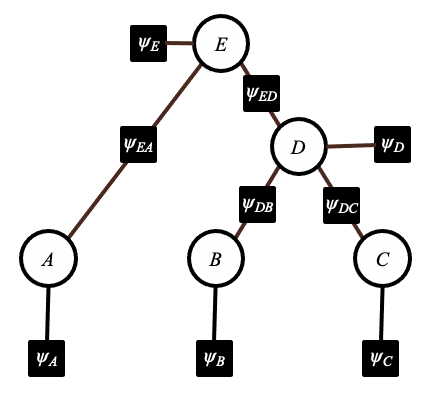
\includegraphics[width=\textwidth]{fig/tree_binary.png}
    \caption{}
    \label{fig:tree_abcde}
\end{figure}

\end{minipage}% This must go next to `\end{minipage}`
\begin{minipage}{.6\textwidth}

\begin{table}[H]
\centering
\begin{subtable}[t]{0.3\textwidth}
    \centering
    \begin{tabular}{cc} 
        \toprule
        $a$ & $\psi_{A}(a)$ \\
        \midrule
        0 & 1 \\
        1 & 2 \\ 
        \bottomrule
    \end{tabular}
\end{subtable}
~
\begin{subtable}[t]{0.3\textwidth}
    \centering
    \begin{tabular}{cc} 
        \toprule
        $b$ & $\psi_{B}(b)$ \\
        \midrule
        0 & 2 \\
        1 & 1 \\ 
        \bottomrule
    \end{tabular}
\end{subtable}
~
\begin{subtable}[t]{0.3\textwidth}
    \centering
    \begin{tabular}{cc} 
        \toprule
        $c$ & $\psi_{C}(c)$ \\
        \midrule
        0 & 1 \\
        1 & 1 \\ 
        \bottomrule
    \end{tabular}
\end{subtable}
\end{table}
\begin{table}[H]
\centering
\begin{subtable}[t]{0.3\textwidth}
    \centering
    \begin{tabular}{cc} 
        \toprule
        $d$ & $\psi_{D}(d)$ \\
        \midrule
        0 & 1 \\
        1 & 1 \\ 
        \bottomrule
    \end{tabular}
\end{subtable}
~
\begin{subtable}[t]{0.3\textwidth}
    \centering
    \begin{tabular}{cc} 
        \toprule
        $e$ & $\psi_{E}(e)$ \\
        \midrule
        0 & 1 \\
        1 & 2 \\ 
        \bottomrule
    \end{tabular}
\end{subtable}
\end{table}
\begin{table}[H]
    \centering
    \begin{subtable}[t]{0.35\textwidth}
    \centering
    \begin{tabular}{ccc} 
        \toprule
        $a$ & $e$ & $\psi_{EA}(a,e)$ \\
        \midrule
        0 & 0 & 1 \\
        0 & 1 & 1 \\
        1 & 0 & 1 \\
        1 & 1 & 1 \\
        \bottomrule
    \end{tabular}
\end{subtable}
~
    \begin{subtable}[t]{0.35\textwidth}
    \centering
    \begin{tabular}{ccc} 
        \toprule
        $d$ & $e$ & $\psi_{ED}(d,e)$ \\
        \midrule
        0 & 0 & 1 \\
        0 & 1 & 1 \\
        1 & 0 & 2 \\
        1 & 1 & 1 \\
        \bottomrule
    \end{tabular}
\end{subtable}
\end{table}
\begin{table}[H]
    \centering
    \begin{subtable}[t]{0.35\textwidth}
    \centering
    \begin{tabular}{ccc} 
        \toprule
        $b$ & $d$ & $\psi_{DB}(b,d)$ \\
        \midrule
        0 & 0 & 1 \\
        0 & 1 & 2 \\
        1 & 0 & 1 \\
        1 & 1 & 1 \\
        \bottomrule
    \end{tabular}
\end{subtable}
~
    \begin{subtable}[t]{0.35\textwidth}
    \centering
    \begin{tabular}{ccc} 
        \toprule
        $c$ & $d$ & $\psi_{DC}(c,d)$ \\
        \midrule
        0 & 0 & 1 \\
        0 & 1 & 1 \\
        1 & 0 & 1 \\
        1 & 1 & 3 \\
        \bottomrule
    \end{tabular}
\end{subtable}
\end{table}

\end{minipage}


\begin{questions}

\begin{EnvFullwidth}
Consider the factor graph in Figure \ref{fig:tree_abcde}. On paper, carry out a run of belief propagation by sending messages first from the leaves $\psi_{A}, \psi_{B}, \psi_{C}$ to the root $\psi_{E}$, and then from the root back to the leaves. Then answer the questions below. Assume all messages are un-normalized.
\end{EnvFullwidth}

\question[1] \textbf{Numerical answer:} What is the message from $A$ to $\psi_{EA}$? 
    \begin{tcolorbox}[fit,height=1cm, width=4cm, blank, borderline={1pt}{-2pt}]
    % STUDENT SOLUTION HERE
    \end{tcolorbox}
    
\question[1] \textbf{Numerical answer:} What is the message from $\psi_{DB}$ to $B$? 
    \begin{tcolorbox}[fit,height=1cm, width=4cm, blank, borderline={1pt}{-2pt}]
    % STUDENT SOLUTION HERE
    \end{tcolorbox}
 
\question[1] \textbf{Numerical answer:} What is the belief at variable $A$? 
    \begin{tcolorbox}[fit,height=1cm, width=4cm, blank, borderline={1pt}{-2pt}]
    % STUDENT SOLUTION HERE
    \end{tcolorbox}
    
\question[1] \textbf{Numerical answer:} What is the belief at variable $B$? 
    \begin{tcolorbox}[fit,height=1cm, width=4cm, blank, borderline={1pt}{-2pt}]
    % STUDENT SOLUTION HERE
    \end{tcolorbox}
    
\question[1] \textbf{Numerical answer:} What is the belief at factor $\psi_{DB}$? 
    \begin{tcolorbox}[fit,height=2cm, width=15cm, blank, borderline={1pt}{-2pt}]
    % STUDENT SOLUTION HERE
    \end{tcolorbox}
    
\question[1] \textbf{Numerical answer:} What is the value of the partition function?
    \begin{tcolorbox}[fit,height=1cm, width=2cm, blank, borderline={1pt}{-2pt}]
    % STUDENT SOLUTION HERE
    \end{tcolorbox}
    
\end{questions}

\clearpage
\subsection{Empirical Questions}

The following questions should be completed after you work through the programming portion of this assignment (Section \ref{sec:code}). 

\begin{questions}

\question[1] \textbf{Select one:} If you feed the inputs shown in Figure \ref{fig:tree_abcde} into your belief propagation module implemented in PyTorch do you get the same answers that you worked out on paper? \textit{(Hint: The correct answer is ``Yes''.)}
    \begin{checkboxes}
     \choice Yes
     \choice No
    \end{checkboxes}

\question[10] Record your model's performance after three epochs on the test set and train set in terms of Cross Entropy (CE) , accuracy (AC) and leaf accuracy (LAC). \emph{Note: Round each numerical value to two significant figures.}


\bgroup
\def\arraystretch{1.5}
\begin{center}
\begin{tabular}{ |c|p{2cm}|p{1cm}| } 
 \hline
 \textbf{Schedule} & \textbf{ Baseline} &  \textbf{CRF } \\
 \hline
Training CE &  & \\ 
 \hline
 Training AC &  &  \\ 
 \hline

Training LAC &  &  \\ 
 \hline

Test AC &  &  \\ 
 \hline

Test LAC &  &  \\ 
 \hline


\end{tabular}
\end{center}
\egroup

\question[10] Plot training and testing cross entropy curves for : \emph{Baseline}, \textit{CRF Model}. Let the $x$-axis ranges over 3 epochs. \emph{Note: Your plot must be machine generated.}

\begin{tcolorbox}[fit,height=12cm, width=15cm, blank, borderline={1pt}{-2pt}]
% STUDENT SOLUTION HERE
\end{tcolorbox}
\end{questions}

\clearpage
\subsection{Collaboration Policy}

    After you have completed all other components of this assignment, report your answers to the collaboration policy questions detailed in the Academic Integrity Policies for this course.
    \begin{enumerate}
        \item Did you receive any help whatsoever from anyone in solving this assignment? If so, include full details including names of people who helped you and the exact nature of help you received.
        
        \begin{tcolorbox}[fit,height=4cm, width=15cm, blank, borderline={1pt}{-2pt},nobeforeafter]
        % Place your solution between the comment lines below.
        % Do not modify the tcolorbox.
        % ----------------------------------------------------
        % STUDENT SOLUTION HERE
        % ----------------------------------------------------
       \end{tcolorbox}
        \item Did you give any help whatsoever to anyone in solving this assignment? If so, include full details including names of people you helped and the exact nature of help you offered.
        
        \begin{tcolorbox}[fit,height=4cm, width=15cm, blank, borderline={1pt}{-2pt},nobeforeafter]
        % Place your solution between the comment lines below.
        % Do not modify the tcolorbox.
        % ----------------------------------------------------
        % STUDENT SOLUTION HERE
        % ----------------------------------------------------
       \end{tcolorbox}
        \item Did you find or come across code that implements any part of this assignment? If so, include full details including the source of the code and how you used it in the assignment.
        
        \begin{tcolorbox}[fit,height=4cm, width=15cm, blank, borderline={1pt}{-2pt},nobeforeafter]
        % Place your solution between the comment lines below.
        % Do not modify the tcolorbox.
        % ----------------------------------------------------
        % STUDENT SOLUTION HERE
        % ----------------------------------------------------
       \end{tcolorbox}
    \end{enumerate}\clearpage
\section{Programming \pts{35}}
\label{sec:code}

Your goal in this assignment is to implement a CRF belief propagation algorithm for  constituency parsing. Given the structure of the tree, you will implement a model to label the nodes with the appropriate tag. Your solution must be implemented in \textbf{PyTorch} using the data files we have provided. We have also provided template code for you to use.

\fullwidth{\subsection{Background: The Constituency Tree Labeling Task}}

Constituency parsing aims to extract a parse tree from a sentence that represents its syntactic structure according to a phrase structure grammar. Terminals are the words in the sentence, non-terminals in the tree are types of phrases, and the edges are unlabeled. The pre-terminals (i.e. nodes just above the leaves, aka words) are called part-of-speech tags. The other non-terminals are clause or phrase level tags. For more information on tags, look \href{http://www.surdeanu.info/mihai/teaching/ista555-fall13/readings/PennTreebankConstituents.html}{here}. Throughout this assignment, we use \textit{nodes} to refer to the set of all non-terminals.

\begin{figure}[h]
\centering
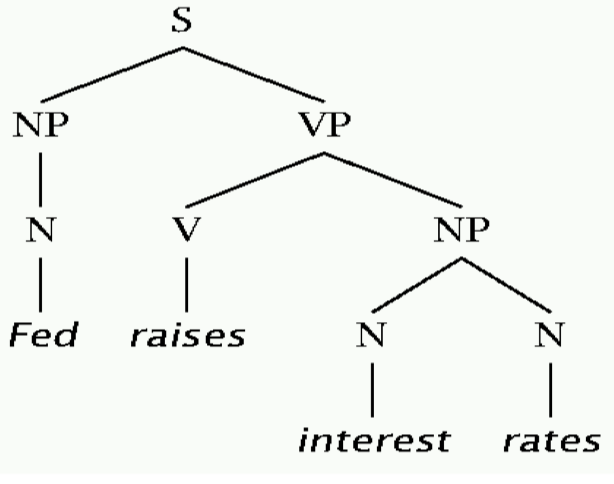
\includegraphics[width=0.50\linewidth]{fig/parsetree.png}
\caption{A parse tree with eight non-terminals: four part-of-speech tags (N, V, N, N) and four phrase-level tags (NP, VP, NP, S).}
\label{overflow}
\end{figure}

In this assignment, we will assume that for each example, the \emph{branching structure} of the tree is \emph{known}, but the tags are not. Given the structure, our goal is to successfully predict the appropriate tag for each node in the tree. We define the accuracy of the model as the average accuracy over all examples where each example consists of a tree structure with $T$ nodes and $L$ leaf nodes. Accuracy for a single tree is defined as:
$$ \text{Acc} = \frac{\text{number of correctly predicted nodes }}{ T}$$
Note that this accuracy is computed across all nodes in the graph. In practice, however, we may particularly care about the POS tags corresponding to each word in the sentence. Thus, we define leaf accuracy as:
$$ \text{Leaf Acc} = \frac{\text{number of correctly predicted leaf nodes }}{L}$$

\clearpage
\fullwidth{\subsection{Background: The Data}}

We have provided a pre-processed version of Penn Tree Bank with {\color{red}13,000} examples, divided into {\color{red}10,000 training examples \lstinline{ptb-train-10000.txt}, 1,000 development examples \lstinline{ptb-dev-1000.txt}, and 2,000 test examples \lstinline{ptb-test-2000.txt}}. Each line consists of one tree. For example, the tree shown above would be encoded as:

\noindent
\lstinline{(S (NP (N Fed)) (VP (V raises) (NP (N interest) (N rates))))}

The trees have already been binarized such that each node has at most two children.
%
We have provided \textbf{starter code} to read each line into an NLTK tree data structure, and a custom tree structure, which you can modify. Note that some functions below have already been implemented for you, however it is your responsibility to read through the code carefully and understand how each function works, because they will be important for later functions that you will have to implement.

The task has the following input/output:
\begin{itemize}
    \item \emph{Given Input:} An input sentence and the associated skeleton of its constituency parse tree
    \item \emph{Predicted Output:} The labels of the non terminals in the parse tree
\end{itemize}

\fullwidth{\subsection{Baseline Model: LSTM with independent tag predictions}}

\begin{figure}[h]
\centering
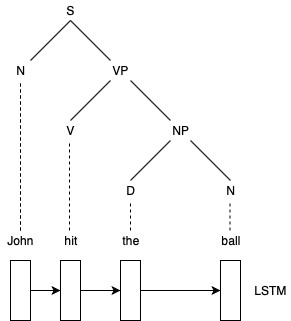
\includegraphics[width=0.3\linewidth]{fig/baseline.png}
\caption{Baseline model using a unidirectional LSTM.}
\label{learned_interp}
\end{figure}

In this section, we have implemented a working baseline LSTM model. Starter code for the model can be found in \verb|baseline_template.py|. As previously mentioned, you are responsible for reading through and understanding this code, because it will help make implementation of the main model easier. Below is an outline/description of the starter code given.

First, we use a torch.nn.Embedding layer to convert our sentence to a tensor representation. Then, we use an LSTM layer (torch.nn.LSTM) to output a ``hidden state" for each node. For the leaf nodes (i.e. nodes corresponding to each token in the sentence), this hidden state is simply the corresponding output of the LSTM. For intermediate nodes, we use a linear layer on the concatenation of the hidden states of the left and the right child. {\color{red} If there is only one child, we concatenate its hidden state with itself.} We use the direct child nodes, \textit{not} the leftmost descendent and rightmost descendent. The output should be a distributions over tags. We can then train the model using cross entropy loss.

Our implementation has a single-layer unidirectional LSTM which outputs a hidden state of dimension 128. The embedding size should be 256. The optimizer should be set to be Adam with a learning rate of 0.0001. Due to the complexity associated with building the tree and computing its potentials, we use a batch size of 1.
% Your program should be able to run on a laptop without GPUs due to the simplicity of the model. 
 
\fullwidth{\subsection{Main Model: LSTM + CRF}}

In this section, you will implement a CRF layer on top of an LSTM representation (Figure \ref{learned_interp}). This will involve computing the unary potentials (a.k.a. factors) corresponding to each node and binary potentials corresponding to each edge in the tree. For an example of unary and binary potentials, see problem A.3. Starter code can be found in \verb|lstm_crf_template.py|. Below is an outline of the model, note that to make the assignment more manageable we have given parts of the implementation to you in the starter code (again it is your responsibility to read through these implementations to understand what the code is doing and for easier implementation of the TODOs). All programming portions that you are required to carry out are marked with TODOs in the starter code.

\begin{enumerate}
    \item \textbf{Representation of potentials.} Instead of keeping an explicit lookup table for the unary and binary potentials, these potentials will be computed by applying a linear layer to the LSTM hidden representation computed for each node (or in the case of binary potentials, concatenation of hidden representations). We compute a unary potential for every node in the graph and an edge potential for every edge. Note that the dotted lines in Figure \ref{learned_interp} do not count as edges. 

    To ensure that the potentials are positive and to provide better numerical stability, we assume that the output of the linear layer is the \emph{logarithm} of the potentials. From there, \textbf{all further computation should be carried out in logspace}.
    
    \item \textbf{Belief propagation.} Now that you've set up the unary and binary potentials, it's time to implement belief propagation. The sum-product belief propagation algorithm proceeds as follows:
    % (a) sending messages from the leaves to the root, (b) sending messages from the root to the leaves, (c) computing the unnormalized marginals (i.e. beliefs), and (d) normalizing the beliefs to return the exact marginals.
    \begin{enumerate}
        \item \emph{Send messages from the leaves to the root.}
        
        As our implementation is a pairwise MRF, we can send messages from node to node directly. Hence, we don't need to calculate intermediate factor node messages. We compute each message as:
    $$m_{i \rightarrow j}(y_j) = \sum_{y_i} \phi_i(y_i) \phi_{ij}(y_i, y_j) \prod_{k \in N(i) \setminus j} m_{k \rightarrow i}(y_i)$$
        
        for an acyclic undirected graphical model defined by $G = (V, E)$ where each element $i \in V$ of the vertex set is an index with a corresponding variable $y_i$ for that node, and $\Nc(i)$ are the neighbors of a node $i$. Messages sent from one variable $y_i$ to another variable $y_j$ is denoted as $m_{i \rightarrow j}(y_j)$.
        % Starting at the leaves, compute the factor and variable messages to be sent upward. Recall that factor messages are computed as:
        % $$\mu_{\alpha \rightarrow i}(x_i) = \sum_{x_\alpha:x_\alpha[i] = x_i}\psi_\alpha(x_\alpha)\prod_{j\in\Nc(\alpha)\setminus i}\mu_{j\rightarrow\alpha}(x_{\alpha}[j])$$
        
        % where the message is being sent from factor $\alpha$ to node $i$, and a matrix-vector product is being computed between the binary factor $\psi_{\alpha}(x_\alpha)$ and the product of incoming messages to $\alpha$. A variable message is computed as:
        % $$\mu_{i \rightarrow \alpha}(x_i) = \prod_{\beta \in \Nc(i)\setminus\alpha}\mu_{\beta\rightarrow i}(x_i)$$
        % where the message is being sent from variable $i$ to factor $\alpha$.
        
%         $$p(\yv) = \frac{1}{Z} \prod_{i \in V} \phi_i(y_i) \prod_{(i,j) \in E} \phi_{ij}(y_i, y_j)$$
% where $\phi_i$ is the potential function for node $i$ and $\phi_{ij}$ the potential for edge $(i,j)$.
        
        
        \item \emph{Send messages from the root to the leaves}: After having computed all messages to send upwards to the root, we can re-use some of these messages when sending messages downward from the root.  
        \item \emph{Compute beliefs}: Given these messages, we are able to compute the beliefs and hence the marginals at each node.
        Variable beliefs can be computed as:
    $$b_i(y_i) = \phi_i(y_i) \prod_{j \in N(i)} m_{j \rightarrow i}(y_i)$$.
    Then variable marginals can be computed as:
    $$p(y_i = k) = \frac{b_i(k)}{\sum_{l \in \Yc} b_i(l)}$$
    \end{enumerate}

    \item \textbf{Useful trick: logsumexp} When numbers are too small or too large, precision can be lost to floating point errors and overflow errors can occur. To circumvent this numerical stability issue, we can compute all messages and potentials in the log space. Multiplication operations on messages would then become addition of log messages, since $\log(ab) = \log(a) + \log(b)$. Addition of messages can be done using the logsumexp operation. Available in pytorch as torch.logsumexp, this function is equivalent to exponentiating the elements of a tensor, summing them along a specified dimension, and then taking the log to put everything back in logspace.
    
    \item \textbf{Loss function: negative log-likelihood.} The loss function should be the negative log-likelihood (NLL), computed from the CRF potentials. This can be done for each sample by looking up and adding up the potentials associated with each node's true label, and subtracting out the partition function. (Hint: How do you compute the partition function from your log belief? Can you think of any sanity checks that can come from the computing the partition function?) 
    
    \item \textbf{Computing accuracy.} To help evaluate your model, compute the accuracy for each tree as well as the accuracy among the leaves. To do so, predict the tag with highest marginal probability for each node, and compare against the true labels. 
    % This method of decoding is equivalent to performing MBR (minimum bayes risk) decoding with Hamming loss.
\end{enumerate}

\paragraph{Additional details:} Again, use a hidden dimension of 128 and embedding dimension of 256. Use the Adam optimizer with learning rate 0.0001.


\fullwidth{\subsection{Code Submission \pts{35}}}
You must submit all of your code to the appropriate slot on Gradescope. 

\end{document}